
% ----------------------------------------------------------
% Introdução (exemplo de capítulo sem numeração, mas presente no Sumário)
% ----------------------------------------------------------
\chapter[Introdução]{Introdução}

  \section{1$^{\circ}$ Sprint}
O primeiro sprint consistiu na preparação do repositório do projeto, com a instalação dos seguintes
    FrameWorks: Code Climate, Cucumber, Jest, Travis CI. Além da configuração dessas ferramentas,
    foi desenvolvido o primeiro esboço do projeto do projeto para inserção no Heroku e teste da configuração.
    Neste esboço, foi criado a Home do site e o arquivo node.js principal. Para a parte de ES4A4,
    foi criado o projeto no PivotalTracker, a fim de inserirmos as User Stories.

    \subsection{Criação do Repositório no Git}
    O primeiro passo tomado pela equipe foi a criação do repositório no Git. Para isso, o integrantes
    Guilherme Leão criou o repositório no GitHub, e posteriormente adicionou todos os membros
    da equipe e o professor de ES4A4, Daniel Morais.\\
    \begin{figure}[!htb]
        \centering
        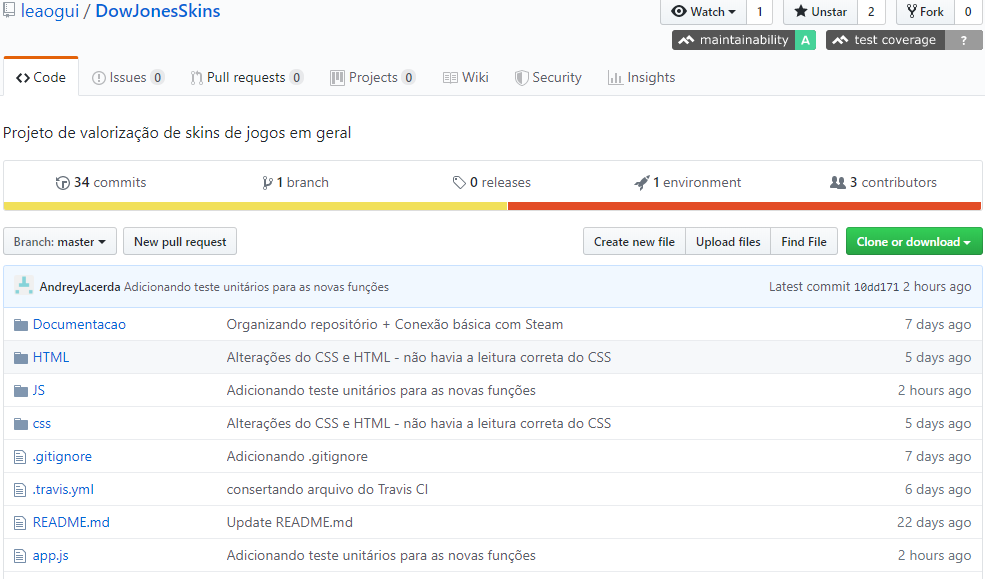
\includegraphics[scale=0.6]{Imagens/Repositorio.png}
        \caption{Repositório do Projeto no GitHub}
    \end{figure}

    \subsection{Instalação dos Frameworks}
    Dentro da pasta raíz do projeto, executamos o comando 'npm init' via CMD. Para isso, instalamos o Node.js
    em nossas máquinas. Este comando criou três arquivos: node\_modules, que consiste no diretório onde todos
    os módulos e bibliotecas utilizadas são salvas; package.json, que consiste em um 'arquivo de configuração',
    possuindo informações sobre a execução do project; package-lock.json, que consiste em um arquivo que salva
    informações de todas as biliotecas e dependencias instaladas no projeto.
    
    Com esses três arquivos criados, instalamos o Jest, a partir do comando 'npm install jest', e o Cucumber, a partir
    do comando 'npm install cucumber'. Ambos os frameworks são utilizados para testes.

    Após instalarmos os dois frameworks para o node.js, instalamos os dois frameworks para o próprio repositório do GitHub.
    O primeiro foi o CodeClimate. Para isso, o dono do repositório instalou a extensão CodeClimate no navegador,
    e posteriormente entrou no git do projeto. Dentro do GitHub do projeto, uma opção apareceu para adicionar
    o projeto ao CodeClimate. Após clicar na opção, o repositório foi lido e adicionado ao CodeClimate, 
    que agora é o plugin de avaliação de código do repositório.

    Após isso, o dono do repositório instalou o Travis CI pelo próprio 'GitHub MarketPlace'. Este framework ainda será melhor explorado,
    por enquanto apenas foi instalado.

    \subsection{Criação e configuração do Heroku}
    Para criarmos o app no Heroku, instalamos o Heroku CLI em nossas máquinas. Com ele instalado, executamos o comando
    'heroku create'. Após criar o Heroku App, entramos no web do Heroku, fizemos o login e configuramos o deploy do Heroku
    para que ele seja sincronizado com o 'push' para o repositório no GitHub.\\
    \begin{figure}[!htb]
        \centering
        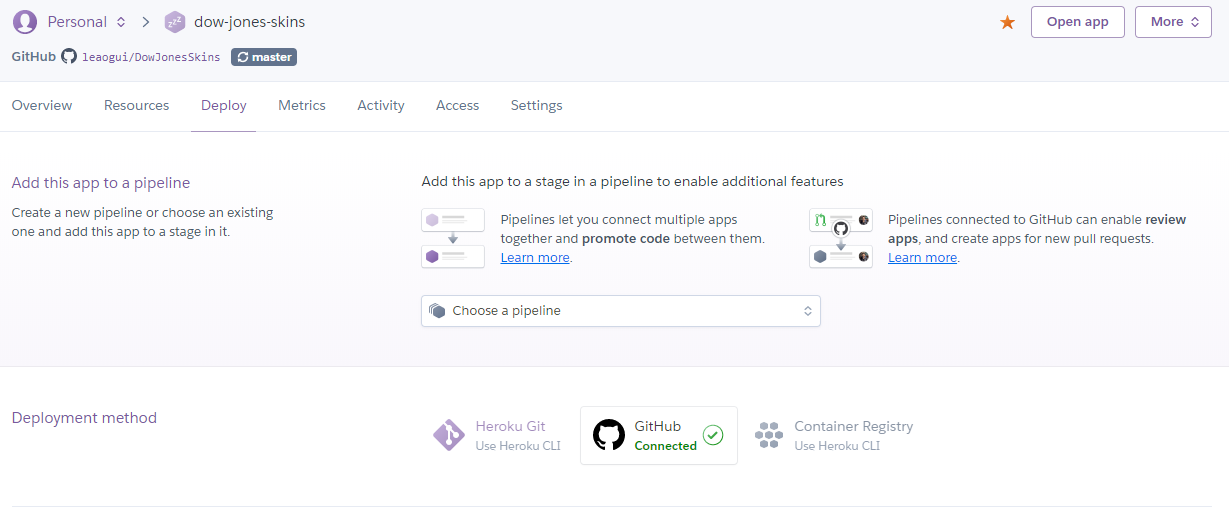
\includegraphics[scale=0.5]{Imagens/Heroku.png}
        \caption{App do Projeto no Heroku}
    \end{figure}

    \subsection{Home.html + app.js}
    Para criar o esboço da Home do projeto, utilizamos HTML, JS e CSS. Para estilização, utilizamos o Bulma,
    que consiste num FrameWork de CSS. Separamos cada arquivo em pastas baseadas em suas extensões. 
    Com isso, criamos uma pasta HTMl, uma CSS e uma JS. Na pasta CSS, jogamos o .min.css do Bulma, para que 
    pudessemos utilizá-lo.

    Com a Home criada, partimos para o primeiro contato com o login via Steam. Para isso, utilizamos a API
    da Steam para Node.JS. No arquivos app.js, que consiste no arquivo 'main', criamos todas as rotas
    e executamos o app via express. Neste arquivo, colocamos as rotas da API Steam, além de configurar
    o middleware, informação a API Key e domínio. Como executaremos tanto em local como no Heroku, modularizamos
    em vários arquivos JS com functions que realizam essa troca de domínio, porta e API Key, já que temos
    uma key apra cada domínio (local e Heroku). 

    Para esas funções foram criadas testes unitários utilizando o Jest. Esses testes estão na subpasta 'tests' 
    dentro da pasta 'JS'.

    Com tudo isso feito, finalizamos a parte de desenvolvimento.\\
    \begin{figure}[!htb]
        \centering
        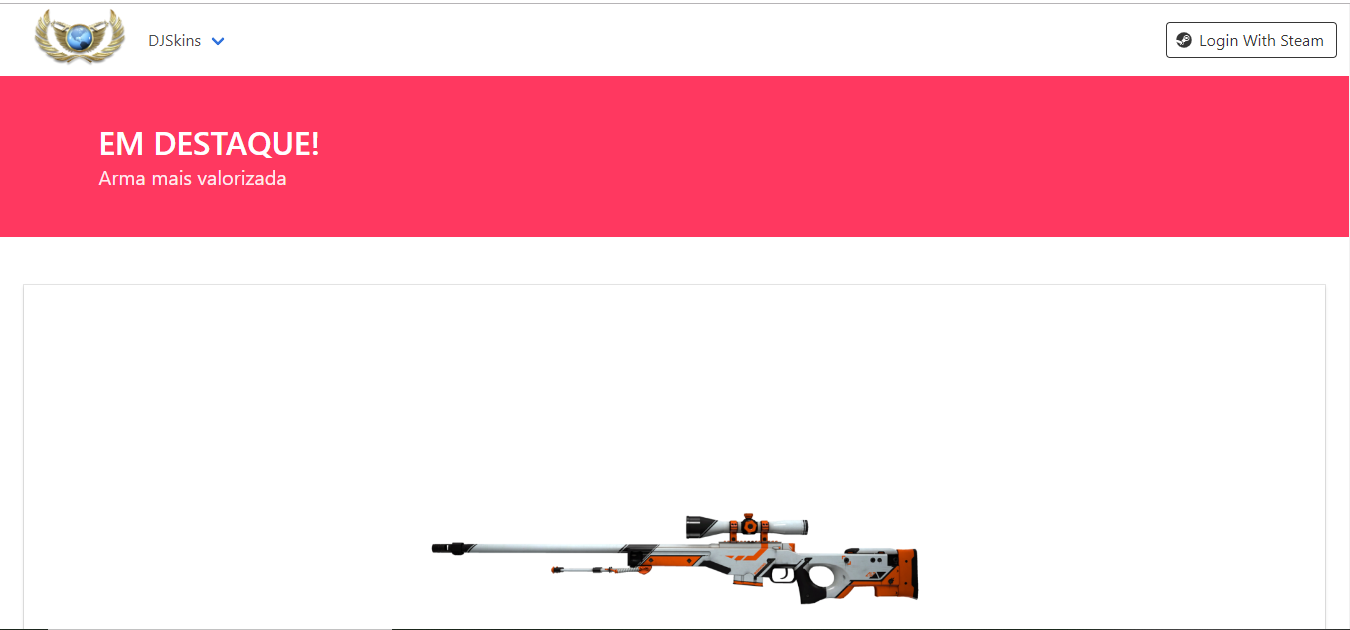
\includegraphics[scale=0.5]{Imagens/Home.png}
        \caption{Esboço da Home pronto}
    \end{figure}

    \subsection{Engenharia de Software}
    No PivotalTracker criado pelo professor Daniel, inserimos as primeiras User Stories. Essas Stories consistem 
    nas principais funcionalidades de usuários que conseguimos identificar e dividir até então. Após inserirmos, 
    Demos a pontuação para cada uma, a partir de um debate, onde o integrante que deu a menor nota defendia seu argumento 
    junto ao integrante de deu a maior nota. O melhor argumento decide a nota.

    Após isso, organizamos a prioridade e dependencias de cada User Story, além de jogarmos uma no IceBox, que 
    consistia na funcionalidade de integrar o site com o PayPal.\\
    \begin{figure}[!htb]
        \centering
        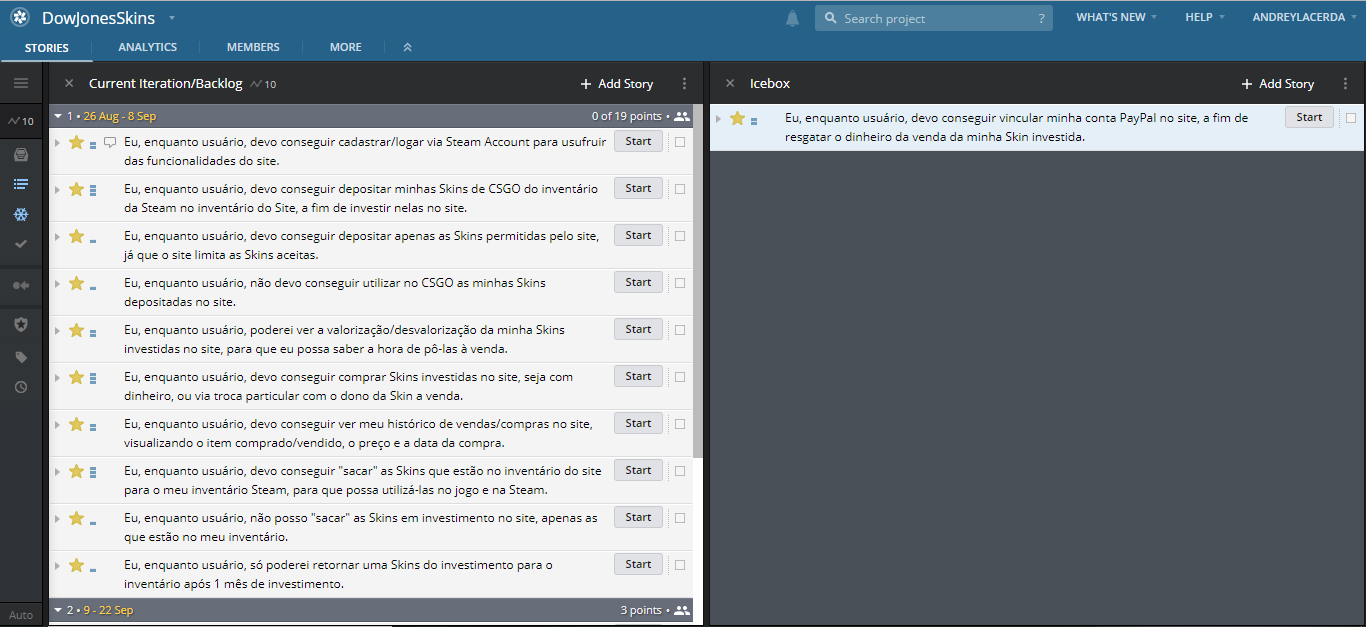
\includegraphics[scale=0.4]{Imagens/Pivotal1.png}
        \caption{PivotalTracker no 1$^{\circ}$ Sprint}
    \end{figure}

    \section{2$^{\circ}$ Sprint}
    \subsection{Descrevendo as features com Cucumber}
    Com as User Stories definidas, o passo seguinte foi esboçar todas as features utilizando o ideal do BDD 
    e utilizando o Cucumber para isso. Com isso, baseando-nos no projeto exemplo mostrado pelo professor Daniel, 
    mais a própria documentação do Cucumber, descrevemos os possíveis cenários de todas as User Stories até então.
    
    Como Dito anteriormente, para isso utilizamos a sintaxe do Cucumber, e separamos acada feature em um arquivo diferente, 
    e salvamos em uma pasta separada, chamada 'Features'. 
    Como sintaxe, declaramos cada User Storie como Feature, descrevemos ela, informamos o Background, e assim os Scenarios.

    \subsection{Testando cadastro/login com Postgre do Heroku}
    Para começar o sistema de cadastro/login, adicionamos o add-ons do PostGre ao Heroku via Heroku CLI. Para isso, 
    usamos o comando 'npm install pg' para instalar o Postgres do projeto. Após isso, adicionamos o add-on do Postgre 
    Heroku via CMD, com comando 'heroku addons:create heroku-postgresql:hobby-dev'. Após isso, seguimos os passos 
    que estão na documentação do Heroku Postgre, encontrada em 'https://devcenter.heroku.com/articles/heroku-postgresql'.

    Após isso, criamos as tabelas via CMD, usando comando 'heroku psql' e adicionando todas as linhas de comando sql.
    Tendo a conexão estável e as tabelas criadas, criamos uma classe chamada 'UserCRUD', e nela utilizamos o json 
    enviado pela Steam após conexão para salvar um Usuário no banco de dados.

    Nessa classe, a função signUp() recebe o json da Steam, conecta ao banco de dados e verifica se este usuário 
    já foi cadastro. Se sim, mais nada é feito, mas caso contrário, o usuário é inserido no banco de dados.
    Tendo isso feito, finalizamos a primeira parte do sistema de cadastro/login.

    \subsection{Estabelecendo Sessão}
    A fim de estabelecer o sistema de login, decidimos utilizar sessão para bloquear o acesso de usuário a 
    determinadas páginas do site. Para isso, utilizamos a constante Session da biblioteca 'Express', que está 
    sendo utlizada para instanciar um Servidor Web.

    Utilizamos o comando app.use() para usar o Session. Neste etapa, inserimos um id para a sessão dentro do 
    parâmetro de inicialização 'secret', e colocamos false nos outros dois itens de inicialização, saveUninitialized e resave, que, 
    após pesquisar, percebemos que não faria sentido algum.

    Após isso, colocamos dentro da página '/verify' a criação da sessão de acordo com o login do usuário na Steam. 
    Com o usuário autenticado via Steam, utilizamos o comando 'req.session.user' e atribuimos o JSON fornecido pela Steam 
    à essa constante.

    Com isso, criamos nossa sessão para cada usuário logado, e após isso, para bloquear o acesso à páginas sem que o user 
    esteja logado, inserimos um 'IF' em cada get do servidor (ignorando a /index e a /login). Dentro do IF, 
    inserimos '!req.session.user', mostrando que caso não exista ression, o usuário deverá ser redirecionado para a 
    tela de login da Steam, finalizando assim o ideal de sessão do site. 

    \subsection{Visualizando o inventário Steam do usário}
    Para obter acesso ao inventário Steam do usário logado, utilizamos da biblioteca 'steam-inventory-api'. 
    Inicializamos o serviço da API quando o servidor sobe. Após isso, quando o usuário se loga na Steam, ele é redirecionado para o '/verify' onde, 
    além de instanciarmos a sessão descrita anteriormente, passamos a visualizar os itens de seu inventário.
    
    Para isso, pegamos a steamId do usuário de dentro do JSON fornecido pela Steam e inserimos como um dos diversos parâmetros da API de 
    inventário. Utilizamos constantes para facilitar o preenchimentos dos outros parâmetros de inicialização, seguindo como base o 
    exemplo de uso da API fornecido em 'https://www.npmjs.com/package/steam-inventory-api'.

    Com isso, ao logar no Steam, o sistema consegue capturar todos os itens trocáveis do inventário do usário, 
    além de filtrar para o jogo 'CSGO'.


    \section{3$^{\circ}$ Sprint}
    \subsection{Peronalização via Cookie}
    A fim personalizar a tela do usuário logado, cookies foram utilizados para 
    exibir seu avatar e seu username. Para isso, o JSON disponibilizado pela steam logo 
    após a autenticação do usuário é salvo no cookie e posteriormente resgatado por duas 
    funções JavaScript encarregadas de resgatar o avatar e o username do user.

    Com isso, o avatar do usuário foi printado na navbar de todas as telas, enquanto logado, enquanto seu nome 
    aparece na página 'Minha Conta'.

    \subsection{Template Engine Handlebars}
    Conforme o projeto foi evoluindo, usa complexidade foi aparecendo. Sabendo que seria necessário o retorno 
    de muita informação do banco de dados para a tela da aplicação, além de muitas regras que resultariam 
    em manipulação do banco, tornou-se necessária a utilização de um Template Engine, tornando a aplicação 
    inteiramente back-end. 
    
    Diante disso, o ‘Handlebars’ foi instalado no sistema e marcado como template engine. Após isso, todos 
    os HTMls desenvolvidos até então foram trocados para Handlebars, e as devidas alterações no back-end 
    foram realizadas.
    
    O HBS foi a escolha por conta de sua natureza totalmente virada para o Node.js, o qual foi utilizado 
    para o back-end inteiro, e por conta de seu fácil aprendizado e resultado que solucionaria os 
    problemas do projeto.

    \section{4$^{\circ}$ Sprint}
    \subsection{Mecânica de Depósito e Saque de Skins}
    A fim de criar a mecânica de deposito e saque de skins, a API ‘steam-inventory’ foi utilizada, 
    junto a algumas funções próprias.
    
    Ao acessar o próprio inventário do DJS, a API ‘steam-inventory’ é utilizada, retornando todas as 
    skins trocáveis de Counter-Strike: Global Offensive. Com essa informação, o nome de tais skins são 
    printadas na tela do usuário em uma coluna a esquerda da tela, enquanto apenas as aceitadas pelo site 
    são printadas na coluna do meio. Na coluna a direita, por sua vez, foi utilizada para printar as 
    skins já depositadas no site pelo usuário. 
    
    Com todas as informações na tela, botões foram adicionados. Na coluna do meio, botões que chamam 
    uma função para investir a skin clicada foram adicionados, enquanto na coluna a direita, botões 
    para sacar skin e investir na skin foram adicionados. A coluna a esquerda ficou apenas com nomes 
    de skins.
    
    Os botões chamam funções, que por sua vez, realizam as devias validações e manipulações no banco 
    de dados, possibilitando assim o mecanismo de deposito e saque.
    
    Devido a burocracias com a Steam, não foi possível criar uma conta para realizar as trocas reais 
    de skins. Com isso, ao depositar uma skin, tal skin não some do inventário real do usuário, 
    apenas é mapeado para dentro do inventário do DJS. A mesma coisa para o saque, em que a 
    skin é realmente enviada para a Steam, mas sim apenas retirada do inventário do DJS, 
    simulando tal troca.

    \subsection{Mecânica de Investimento de Skins}
    A fim de investir na skin, mecanismo core da aplicação, o botão na ‘Investir’ foi criado 
    para cada skin no inventário DJS do usuário. Ao clicar no botão, uma função é invocada, 
    que realiza a confirmação do investimento da skin, marcando a data do investimento.
    Com a data marcada, o usuário não pode retirar o investimento até bater 31 dias, que 
    consiste em outro User Story do projeto.

    A fim de simular a flutuação de valores das skins do mercado, ao investir em uma skin, 
    caso a skin investida é a primeira no sistema inteiro, seu valor aumenta 
    15\%. Caso contrário, cai 3\%.

    \section{5$^{\circ}$ Sprint}
    \subsection{Mecânica de Carteira}
    Após a implementação do deposito, saque e investimento de skins, a mecânica de carteira foi 
    desenvolvida para possibilitar a compra de skins. Para isso, foi criado uma sessão ‘Carteira’, e 
    uma coluna ‘saldo’ na tabela ‘usuario’ do Postgresql. 
    
    Ao clicar em ‘Depositar’ na sessão de ‘Carteira’, automaticamente R\$15 creditados em seu ‘saldo’, 
    realizando um UPDATE no banco de dados. Ao informar uma quantia a sacar e clicar em ‘Retirar’, tal 
    quantia é validada com o saldo. Se o saldo for maior ou igual a quantia, tal valor é debitado do 
    saldo, realizando outro UPDATE no banco de dados.

    \subsection{Mecânica de Compra de Skins e Histórico de Vendas}
    Para o mecanismo de compra, foi criado a sessão ‘DayTrade’, em que o usuário 
    acessará para ver todas as skins investidas no site e seu determinado preço, além 
    de ver seus próprios investimentos, possibilitando o cancelamento de algum deles, 
    caso tenham mais de 31 dias.
    
    Com isso, ao encontrar um skin que deseja, o usuário clica em ‘Comprar’, e uma função é 
    chamada para validar a compra. Se a compra for válida, o usuário comprador recebe a skin 
    do usuário “vendedor” que está a mais tempo com o investimento aberto. Com isso, do saldo do 
    comprador é debitado o valor da skin, enquanto do saldo do vendedor é creditado tal valor. 
    
    Além disso, um histórico de vendas é criado, marcando assim o nome do vendedor/comprador, as 
    informações da skin comprada e a data da compra. Tal histórico também pode ser visto na tela 
    ‘DayTrade’.

    \subsection{Testes}
    Após todos os desenvolvimentos serem concluídos e testados pela equipe, o desenvolvimento de 
    teste automatizados foram realizados. Para isso, o framework de testes Jest foi utilizado para 
    o testes unitários e de integração, enquanto o Puppeteer e o Cucumber foram utilizados para os 
    testes End-To-End. 
    
    Ao total, dezesseis testes foram implementados, testando as funcionalidades principais do sistema, 
    evitando qualquer má manipulação de banco de dados e interferência no mecanismo de valorização de
     skins do site.
    
    Além desses testes, uma ferramenta de análise estática foi utilizada no projeto. Tal ferramenta 
    foi o ‘jshint’, e serviu como “cleaner” de “code smells”. A análise estática de 100\% ao final 
    das refatorações requisitadas pela ferramenta.

    \section{User Stories}
    Eu, enquanto usuário, devo conseguir cadastrar/logar via Steam Account para usufruir das 
    funcionalidades do site.

    Eu, enquanto usuário, devo conseguir depositar minhas Skins de CSGO do inventário da Steam no 
    inventário do Site, a fim de investir nelas no site.

    Eu, enquanto usuário, devo conseguir depositar apenas as Skins permitidas pelo site, já que o 
    site limita as Skins aceitas.

    Eu, enquanto usuário, devo conseguir colocar na bolsa uma Skins do meu inventário do site, para 
    que ela possa valorizar/desvalorizar com o tempo.

    Eu, enquanto usuário, não posso "sacar" as Skins em investimento no site, apenas as que estão no 
    meu inventário.

    Eu, enquanto usuário, só poderei retornar uma Skins do investimento para o inventário após 1 mês 
    de investimento.

    Eu, enquanto usuário, devo conseguir "sacar" as Skins que estão no inventário do site para o meu 
    inventário Steam, para que possa utilizá-las no jogo e na Steam.

    Eu, enquanto usuário, devo conseguir ver meu histórico de vendas/compras no site, visualizando o 
    item comprado/vendido, o preço e a data da compra.

    Eu, enquanto usuário, poderei ver a valorização/desvalorização das Skins investidas no site, para 
    que eu possa saber a hora de comprar e vender.

    Eu, enquanto usuário, devo conseguir comprar Skins investidas no site com dinheiro.

